\section{SCGRA Overlay Infrastructure} \label{sec:scgraimplement}
One key idea of QuickDough is to rely on an intermediate SCGRA overlay to improve compilation time of the high-level user application. While the exact design of this SCGRA does not affect the compilation flow, its implementation does have a significant impact on the performance of the generated gateware.
 
\subsection{SCGRA Based FPGA Accelerator}
Figure \ref{fig:scgra-accelerator} is the proposed FPGA accelerator built on top of SCGRA. Its communication interface with the host system follows exactly the typical FPGA acceleration system, while the computation core is a synchronous SCGRA which is esentially an array of homogeneous PEs. The topology of the SCGRA is one of the major design parameters. High dimension topology is preferred for kernels with heavy communication, while low dimension topolpgy is more scalable and can be implemented more efficiently. Currently, 2D Torus with both comparable scalability and communication bandwidth is used in this work. 

On top of the computation array, two address buffers instead of customized logic are provided as the address generator. When the high level application changes within the SCGRA's supporting set, we don't have to develop a new address generator for it and can simply replace its content together with the SCGRA configuration contexte. Therfore, it helps reduce the chance of FPGA implementation and eventually improves the design productivity of the FPGA acceleration framwork. 

While usually the input and output data buffer could store more data than that used by a single SCGRA execution, thus the SCGRA may iterate multiple times before it consumes all the data in input buffer or fills the output buffer. From the perspective of software, it is more convenient to control all the computation involved in the data buffer instead of each SCGRA execution. In this case, we have a control unit called SCGRA Ctrl to make the multiple SCGRA execution transparent to the ACC Ctrl. Now, there are only two single bit signals between the ACC Ctrl and the rest of the accelerator. Then two consecutive registers are applied to separate the clock domain of communication interface and the computation core. The optimized SCGRA could be easily pipelined and work at higher frequency, while the interface needs to handle complex protocol and works at lower frequency.

\begin{figure}[h]
    \center{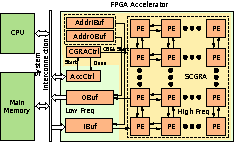
\includegraphics[width=0.8\linewidth]{scgra-accelerator}}
    \caption{SCGRA Accelerator}
    \label{fig:scgra-accelerator}
\end{figure}

\subsection{PE}
In this section, an instance of PE is presented to demonstrate the feasibility of producing high performance gateware. As shown in \figref{fig:pe}, the PE, centring an ALU block, a multiple-port data memory and an instruction ROM, is highly optimized for FPGA implementation. In addition, a load/store path is implemented on the PEs that are responsible for data I/O beyond the FPGA and an Addr Ctrl is employed to start as well reset the SCGRA execution.

\begin{figure}[h]
\center{\includegraphics[width=0.95\linewidth]{pe}}
\caption{PE structure}
\label{fig:pe}
\end{figure}

\subsubsection{Instruction Memory and Data Memory}
The instruction memory stores all the control words of the PE in each cycle. Since its content does not change during runtime, a ROM is used to implement this instruction memory. The content of the ROM is loaded together with the configuration bitstream. The address of the instruction ROM is determined by the Addr Ctrl. Basically, the SCGRA execution will proceed when the start signal is valid, and it will be reset when the start signal is invalid.

Data memory stores intermediate data that can either be forwarded to the PE downstream or be sent to the ALU for calculation. For fully parallelized operation, \emph{at least} four read ports are needed -- three for the ALU and one for data forwarding. Similarly, at least two write ports are needed to store input data from upstream memory and to store the result of the ALU in the same cycle. Although a pair of true dual port memories may seems to be able to satisfy this port requirement, conflicts may arise if the ALU needs to read the data while the data path needs to be written. As a result, a third dual port memory is replicated in the data memory.

Note that data memory here is usually implemented as a multiple port register file in many previous CGRA work. Although register file is even more flexible in terms of parallel reading and writing, the multi-port register file size is limited due to the inefficient hardware implementation. While we have a much larger DFG for scheduling and thus larger temporary storage is required, we eventually use a multi-port data memory instead. 

\subsubsection{ALU}
At the heart of the proposed PE is an ALU designed to cover the computations in target application. \figref{fig:ALU} shows an example design that could support all the operations of our benchmark which is listed in \tabref{tab:operations}. Complpex operations like MULADD/MULSUB are implemented with DSP core directly. Operations with moderate complexity like ADDADD, RSFAND etc. are divided into two stages naturally and hardware block reuse is also considered at the same time. Finally, simple operations that can be done in a single cycle can be put in either stage depending on the pipeline status. Note that MUX in data path has significant influence on timing as well, so small MUX should be inserted properly and large MUX should be avoided. Currently, we just manually optimize the ALU design, but it is possible to automate this step. 

\begin{figure}[h]
\center{\includegraphics[width=0.8\linewidth]{alu}}
\caption{ALU Example}
\label{fig:ALU}
\end{figure} 

\begin{table}[h]
\caption{Operations Involved in The Benchmark}
\label{tab:operations}
\centering
\begin{tabular}{|p{1.5cm}|p{1.5cm}|p{4cm}|}
\hline
Type & Opcode & Expression \\

\hline
MULADD & 0001 & {dst = src0 $times$ src1 + src2} \\

\hline
MULSUB & 0010 & {dst = src0 $times$ src1 - src2} \\

\hline
ADDADD & 0011 & {dst = src0 + src1 + src2} \\

\hline
ADDSUB & 0100 & {dst = src0 + src1 - src2} \\

\hline
SUBSUB & 0101 & {dst = src0 - src1 -src2} \\

\hline 
PHI & 0110 & {dst = src0 ? src1 : src2} \\

\hline
RSFAND & 0111 & {dst = (src0 $>>$ src1) \& src2} \\

\hline
LSFADD & 1000 & {dst = (src0 $<<$ src1) + src2} \\

\hline
ABS & 1001 & {dst = abs(src0)} \\

\hline
GT & 1010 & {dst = (src0 $>$ src1) ? 1 : 0} \\

\hline
LET & 1011 & {dst = (src0 $<=$ src1) ? 1 : 0} \\

\hline
ANDAND & 1100 & {dst = src0 \& src1 \& src2} \\

\hline
\end{tabular}
\end{table}

\subsection{Load/Store Interface}
For the PEs that also serve as I/O interface to the SCGRA, there are also additional load path and store path as shown in \ref{fig:pe}. To keep the balance of the pipeline, an additional pipeline stage is added to chosse between neighboring input and SCGRA input interface. While store path has no influence on the rest of the design. In addition, as load path and store path can be connected to the read port and write port of the I/O buffer at the same time, there is no further customization for input PE or output PE. 

